%%%%%%%%%%%%%%%%%%%%%%%%%%%%%%%%%%%%%%%%%%%%%%%%%%%%%%%%%%%%%%%%%%%%%%%%%%%%
% AGUJournalTemplate.tex: this template file is for articles formatted with LaTeX
%
% This file includes commands and instructions
% given in the order necessary to produce a final output that will
% satisfy AGU requirements, including customized APA reference formatting.
%
% You may copy this file and give it your
% article name, and enter your text.
%
%
% Step 1: Set the \documentclass
%
% There are two options for article format:
%
% PLEASE USE THE DRAFT OPTION TO SUBMIT YOUR PAPERS.
% The draft option produces double spaced output.
%

%% To submit your paper:
\documentclass[draft]{agujournal2019}
%\documentclass[]{agujournal2019}
\usepackage{textcomp}
\usepackage{url} %this package should fix any errors with URLs in refs.
\usepackage{lineno}
\usepackage{setspace}
\usepackage{xcolor}
\linenumbers
%%%%%%%
% As of 2018 we recommend use of the TrackChanges package to mark revisions.
% The trackchanges package adds five new LaTeX commands:
%
%  \note[editor]{The note}
%  \annote[editor]{Text to annotate}{The note}
%  \add[editor]{Text to add}
%  \remove[editor]{Text to remove}
%  \change[editor]{Text to remove}{Text to add}
%
% complete documentation is here: http://trackchanges.sourceforge.net/
%%%%%%%

%\draftfalse

%% Enter journal name below.
%% Choose from this list of Journals:
%
% JGR: Atmospheres
% JGR: Biogeosciences
% JGR: Earth Surface
% JGR: Oceans
% JGR: Planets
% JGR: Solid Earth
% JGR: Space Physics
% Global Biogeochemical Cycles
% Geophysical Research Letters
% Paleoceanography and Paleoclimatology
% Radio Science
% Reviews of Geophysics
% Tectonics
% Space Weather
% Water Resources Research
% Geochemistry, Geophysics, Geosystems
% Journal of Advances in Modeling Earth Systems (JAMES)
% Earth's Future
% Earth and Space Science
% Geohealth
%
% ie, \journalname{Water Resources Research}

\journalname{Tectonics}


\begin{document}

%% ------------------------------------------------------------------------ %%
%  Title
%
% (A title should be specific, informative, and brief. Use
% abbreviations only if they are defined in the abstract. Titles that
% start with general keywords then specific terms are optimized in
% searches)
%
%% ------------------------------------------------------------------------ %%

% Example: \title{This is a test title}

\title{The paleogeography of Laurentia in its early years: new constraints from the Paleoproterozoic East Central Minnesota batholith}

%% ------------------------------------------------------------------------ %%
%
%  AUTHORS AND AFFILIATIONS
%
%% ------------------------------------------------------------------------ %%

% Authors are individuals who have significantly contributed to the
% research and preparation of the article. Group authors are allowed, if
% each author in the group is separately identified in an appendix.)

% List authors by first name or initial followed by last name and
% separated by commas. Use \affil{} to number affiliations, and
% \thanks{} for author notes.
% Additional author notes should be indicated with \thanks{} (for
% example, for current addresses).

% Example: \authors{A. B. Author\affil{1}\thanks{Current address, Antartica}, B. C. Author\affil{2,3}, and D. E.
% Author\affil{3,4}\thanks{Also funded by Monsanto.}}

\authors{Nicholas L. Swanson-Hysell\affil{1},  Margaret S. Avery\affil{1}, Yiming Zhang\affil{1}, Robert J.Sherwood\affil{1}, Eben B. Hodgin\affil{1}, Sarah P. Slotznick\affil{1,2}, C. Brenhin Keller\affil{1,2,3}, David L. Shuster\affil{1,3}, Terry J. Boerboom\affil{4}, Francisco Apen\affil{5}, John M. Cottle\affil{5}}

% \affiliation{1}{First Affiliation}
% \affiliation{2}{Second Affiliation}
% \affiliation{3}{Third Affiliation}
% \affiliation{4}{Fourth Affiliation}

\affiliation{1}{Department of Earth and Planetary Science, University of California, Berkeley, CA, USA}
\affiliation{2}{Department of Earth Sciences, Dartmouth College, Hanover, NH, USA}
\affiliation{3}{Berkeley Geochronology Center, 2455 Ridge Road, Berkeley, CA 94709, USA}
\affiliation{4}{Minnesota Geological Survey, St. Paul, Minnesota, USA}
\affiliation{5}{Department of Earth Science, University of California, Santa Barbara, CA, USA}
%(repeat as many times as is necessary)

%% Corresponding Author:
% Corresponding author mailing address and e-mail address:

% (include name and email addresses of the corresponding author.  More
% than one corresponding author is allowed in this LaTeX file and for
% publication; but only one corresponding author is allowed in our
% editorial system.)

% Example: \correspondingauthor{First and Last Name}{email@address.edu}

\correspondingauthor{Nicholas Swanson-Hysell}{swanson-hysell@berkeley.edu}

%% Keypoints, final entry on title page.

%  List up to three key points (at least one is required)
%  Key Points summarize the main points and conclusions of the article
%  Each must be 100 characters or less with no special characters or punctuation

% Example:
% \begin{keypoints}
% \item	List up to three key points (at least one is required)
% \item	Key Points summarize the main points and conclusions of the article
% \item	Each must be 100 characters or less with no special characters or punctuation
% \end{keypoints}

\begin{keypoints}
\item A new paleomagnetic pole for ca. 1780 Ma diabase dikes of the East Central Minnesota Batholith reconstructs the Superior province to moderately high latitudes.
\item A mild thermal history for the batholith since the Paleoproterozoic is supported by new U-Pb apatite and U-Th-He zircon thermochronology.
\item This paleomagnetic pole establishes the coherency of the amalgamated Laurentia craton following Trans-Hudson orogenesis and supports the NENA connection with Fennoscandia.
\end{keypoints}

%% ------------------------------------------------------------------------ %%
%
%  ABSTRACT
%
% A good abstract will begin with a short description of the problem
% being addressed, briefly describe the new data or analyses, then
% briefly states the main conclusion(s) and how they are supported and
% uncertainties.
%% ------------------------------------------------------------------------ %%

%% \begin{abstract} starts the second page

\begin{abstract}



%The craton of Laurentia assembled in the Paleoproterozoic from its constituent Archean provinces. At the same time that the Super
%
%At the with this assembly, coeval accretionary orogenesis on the southern margin associated with the Penokean orogeny that was followed by subsequent accretionary orogenesis that progressively moved further outboard into the Mesoproterozoic. Following 
%
%While the southeast margin of Laurentia experienced subsequent intervals of accretionary orogenesis, these all occurred outboard from the stabilized lithosphere in the region of the East Central Minnesota Batholith. As a result, it did not experience subsequent tectonothermal events that would have modified the magnetic remanence of the diabase dikes. The exception being the Midcontinent Rift that resulted in the intrusion of dike studied in this work. This dike cross-cuts an ECMB dike and passes a baked contact test. Pyrrhotite 
%
%intrusion of  d
%
%
%numerous interaccetion


\end{abstract}



%% ------------------------------------------------------------------------ %%
%
%  TEXT
%
%% ------------------------------------------------------------------------ %%

%%% Suggested section heads:
% \section{Introduction}
%
% The main text should start with an introduction. Except for short
% manuscripts (such as comments and replies), the text should be divided
% into sections, each with its own heading.

% Headings should be sentence fragments and do not begin with a
% lowercase letter or number. Examples of good headings are:

% \section{Materials and Methods}
% Here is text on Materials and Methods.
%
% \subsection{A descriptive heading about methods}
% More about Methods.
%
% \section{Data} (Or section title might be a descriptive heading about data)
%
% \section{Results} (Or section title might be a descriptive heading about the
% results)
%
% \section{Conclusions}


\section{Introduction} 

In the Orosirian Period of the Paleoproterozoic Era, a series of collisional orogenies led to the amalgamation of Archean provinces to form the core of the Laurentia craton (Fig. \ref{fig:Laurentia_map}; \citeA{Hoffman1988a, Whitmeyer2007a}). The most significant of these orogenies was the ca. 1850 to 1800 Ma Trans-Hudson orogeny associated with the collision between the Superior province and the Churchill province which comprised a composite of the Slave, Hearne and Rae provinces (Fig. \ref{fig:Laurentia_map}; \citeA{Weller2017a}). The rapid Paleoproterozoic amalgamation of Laurentia led to the large persistent area of continental lithosphere that would grow further through accretionary orogenesis subsequently in the Paleoproterozoic Era and through the Mesoproterozoic Era \cite{Whitmeyer2007a}. The terminal closure of the intervening ocean basin between the Superior and composite Slave + Hearne + Rae provinces is interpreted in some paleogeographic models to be associated not only with the assembly of Laurentia, but also with the conjoining of other continents into the hypothesized supercontinent Nuna \cite{Pehrsson2015a}. The history of subsequent orogenesis along the southern to eastern margin of Laurentia (present-day coordinates) indicates that it was a long-lived accretionary margin through the rest of the Paleoproterozoic and into the Mesoproterozoic \cite{Karlstrom2001a, Whitmeyer2007a}. This accretionary margin has been interpreted to have extended beyond Laurentia and have continued onto Baltica and Australia \cite{Karlstrom2001a}. Based on correlation of Archean provinces and Paleoproterozoic orogenic belts, \citeA{Gower1990a} reconstructed Baltica to Laurentia in a position known as the NENA (northern Europe and North America) configuration. This reconstruction is compatible with existing paleomagnetic constraints from ca. 1750 to 1270 Ma \cite{Evans2008a} and these conjoined cratons feature as a major component of the hypothesized Nuna supercontinent \cite{Evans2011a, Zhang2012a}. Additional data that constrains the paleogeographic position of Laurentia from the time just following the Trans-Hudson orogeny can test the hypothesis of the unity of Laurentia's Archean provinces, establish the position of the newly amalgamated Laurentia and thereby enable tests of hypothesized connections with other cratons such as Baltica. This study develops a new paleomagnetic pole for Laurentia from ca. 1780 Ma diabase dikes of the East Central Minnesota Batholith (ECMB) that provides such a constraint.

\begin{figure}[!ht]
\centering
\noindent\includegraphics[width=\textwidth]{Figures/overview_map.pdf}
\caption{\setstretch{0.7}\small{Map of Laurentia showing the location of Archean provinces and younger Proterozoic crust (simplified from \cite{Whitmeyer2007a}). The localities of paleomagnetic poles that constrain Laurentia's position just after its amalgamation are shown with stars including the new pole from this study developed from the East Central Minnesota Batholith (ECMB). The outline of the state of Minnesota around the ECMB red star is the region for the geologic map in the right panel. This map shows interpreted Precambrian geology for the state of Minnesota (simplified from \citeA{Jirsa2012a}) including in regions where covered by Phanerozoic sedimentary cover where the Precambrian bedrock is inferred from geophysical maps and drill core.}}
\label{fig:Laurentia_map}
\end{figure}

\section{Geologic Setting}

Coeval with collisional orogenesis between the assembling Archean provinces that formed Laurentia's core was the ca. 1860 to 1820 Ma accretionary Penokean orogeny along the southern margin of the Superior Province (Fig. \ref{fig:Laurentia_map}; \citeA{Schulz2007a}). Penokean orogenesis resulted from island-arc and microcontinent collisions with the Superior Province that led to metamorphism of Superior Province lithologies and development of a foreland basin \cite{Schulz2007a, Holm2019a}. Following the Penokean orogeny, there was voluminous magmatism within the southwestern Superior Province resulting in the emplacement of the ca. 1780 East Central Minnesota Batholith (ECMB) and other coeval plutons (Fig. \ref{fig:Laurentia_map}; \citeA{Holm2005a, Boerboom2005b, Schmitz2018a}). While the ECMB is dominantly comprised of felsic to intermediate plutons, mafic magmas were also generated and commingled with the more abundant felsic magmas throughout the interval of batholith generation as evidenced by mafic enclaves within some of the plutons \cite{Boerboom2005b, Boerboom2011b, Schmitz2018a}. Mafic melt within the ECMB also led to the emplacement of a set of near-vertical northeast-trending diabase dikes (Fig. \ref{fig:site_map}; \citeA{Boerboom2005b}).  The dikes have chilled margins and are typically 1 to 3 meters wide with widths up to 8 meters \cite{Boerboom2005b}. As with the granites they intrude, the dikes have primary igneous texture and no metamorphic fabric \cite{Boerboom2005b}. These diabase dikes are present within all of the granitoid units of the batholith (e.g., St. Cloud, Foley, and Rockville granites, and Reformatory granodiorite; Fig. \ref{fig:site_map}) with the exception of the youngest Richmond granite. There are also quartz-feldspar porphyry dikes with the same northeast-trending direction as the diabase dikes found in all granitoids also with the exception of the Richmond granite. The Richmond granite has trachytoid magmatic fabric defined by aligned potassium-feldspar phenocrysts that share the same orientation with the northeast-trending dikes \cite{Boerboom2000a} indicating that this orientation is associated with a persistent regional stress field throughout the interval of magma emplacement and dike formation. These field relationships indicate that the quartz-feldspar porphyry and diabase dikes are comagmatic with the batholith. The diabase dikes are constrained to be younger than the St. Cloud Granite (new U-Pb date of 1781.44$\pm$0.51 Ma; 2$\sigma$ uncertainty) which they pervasively intrude, older than the Richmond granite (new U-Pb date of 1776.76$\pm$0.49 Ma) in which they are absent, and similar in age to the quartz-feldspar porphyry dikes (new U-Pb date of 1780.78$\pm$0.45 Ma). The age of the northeast-trending diabase dikes within the ECMB is therefore ca. 1779$\pm$3 Ma.

\begin{figure}[!ht]
\centering
\noindent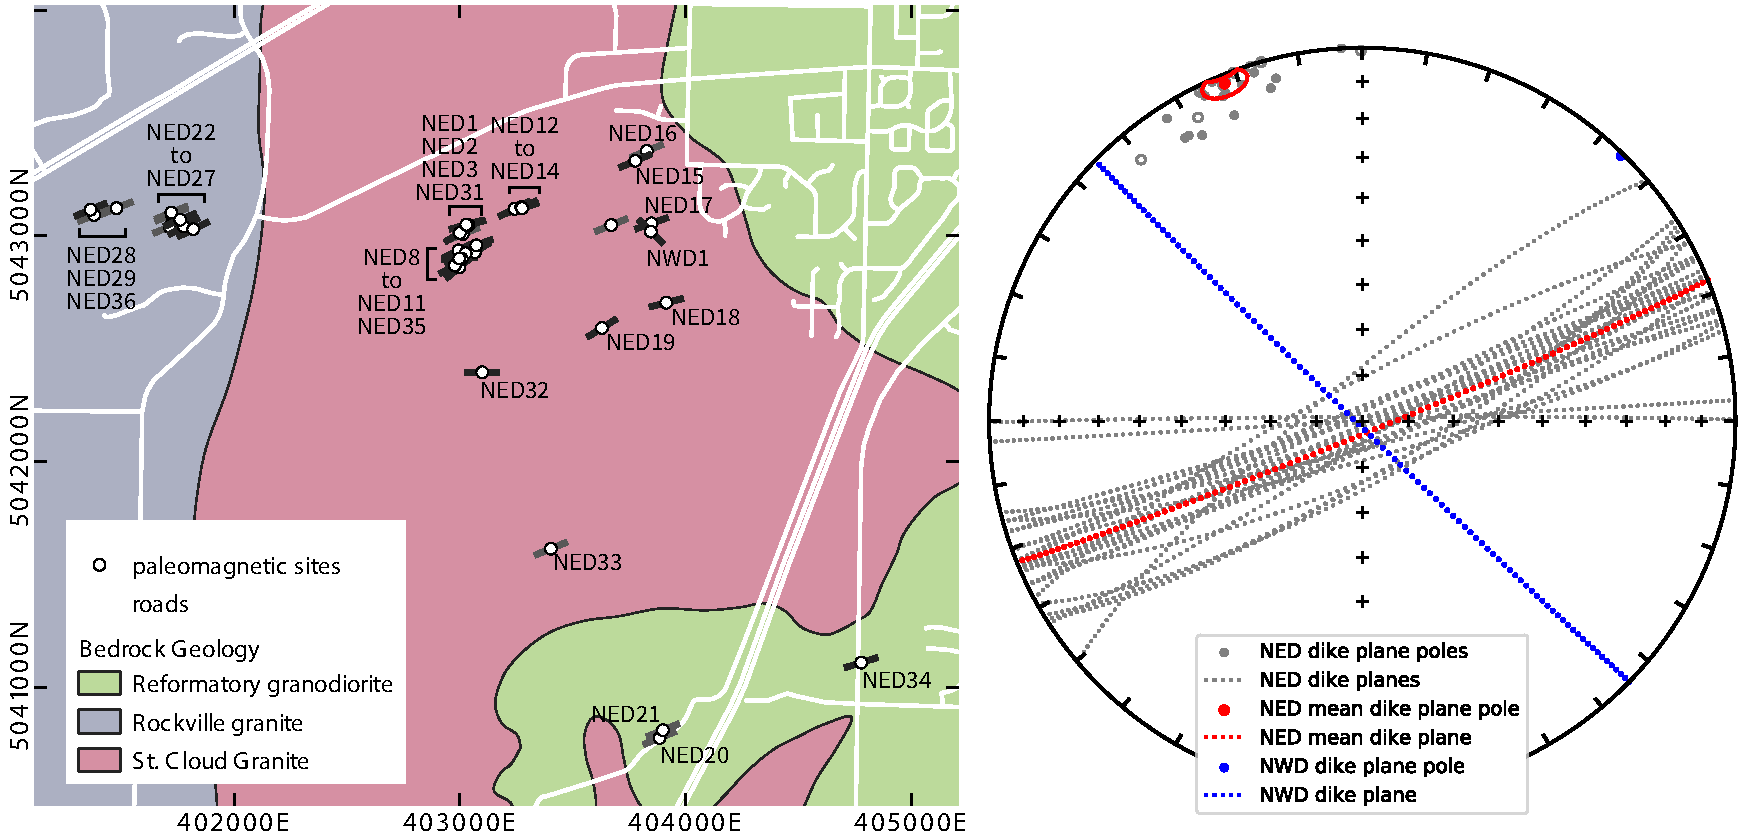
\includegraphics[width=\textwidth]{Figures/site_map.pdf}
\caption{\setstretch{0.7}\small{Left panel: Locations of paleomagnetic sites within the Rockville granite, Reformatory granodiorite and St. Cloud granite of the ECMB (bedrock geology from \citeA{Meyer1995a} and shown in UTM zone 15N WGS 84 coordinate reference system). Within regions of the mapped St. Cloud granite there is more complex interfingering of that granite with the Reformatory granodiorite than is shown. The strikes of the dikes are shown as lines (black when measured on that dike; grey when using the overall mean orientation). Right panel: The orientations of northeast-trending dikes (NED) and the northwest-trending dike (NWD). Each individual dike orientation is the mean of multiple measurements on that dike. The mean of the poles to the NED planes is shown with a red dot and a 95$\%$ confidence ellipse on the mean calculated with Fisher statistics. This confidence ellipse intersects the equator indicating that the mean plane can not be distinguished from vertical.}}
\label{fig:site_map}
\end{figure}

\section*{Paleomagnetic Methods and Results}

Oriented samples were collected and analyzed from 36 of the northeast-trending dikes of the ECMB and one northwest-trending dike (Fig. \ref{fig:site_map}). Each sampled dike constituted a paleomagnetic site in our site naming scheme. These sites were concentrated in and around Stearns County Quarry Park near the city of St. Cloud (Fig. \ref{fig:site_map}). There are two principal modes of exposure of dikes in the region. The first exposure type is pavement outcrops that are glacially-polished from the most recent advance and retreat of the Laurentide ice sheet. The second exposure type is within dimension stone granite quarries that provide fresh three-dimensional exposure of the plutonic lithologies and the diabase dikes. Samples were collected from these dikes with a gas-powered drill and oriented in the field with a Pomeroy orienting fixture. The azimuthal orientations of the cores were determined either through sun or magnetic compass depending on the cloud cover. Sun compass directions were preferentially used when available. Specimens from the oriented samples were analyzed in the UC Berkeley Paleomagnetism lab on a 2G DC-SQUID magnetometer. Samples either underwent stepwise alternating field (AF) or thermal demagnetization. Thermal demagnetization was accomplished using an ASC thermal demagnetizer (residual fields $<$10 nT). AF demagnetization was conducted with inline coils that utilize a Crest Amplifier paired with an Adwin controller to develop a well-controlled waveform. All paleomagnetic data developed in this study are available at the measurement level in the MagIC database (https://www.earthref.org/ MagIC/ doi/ INSERTDOI). \textit{for the purposes of review, all data are available here: \url{https://github.com/Swanson-Hysell-Group/ECMB_project}}

\begin{figure}[!ht]
\noindent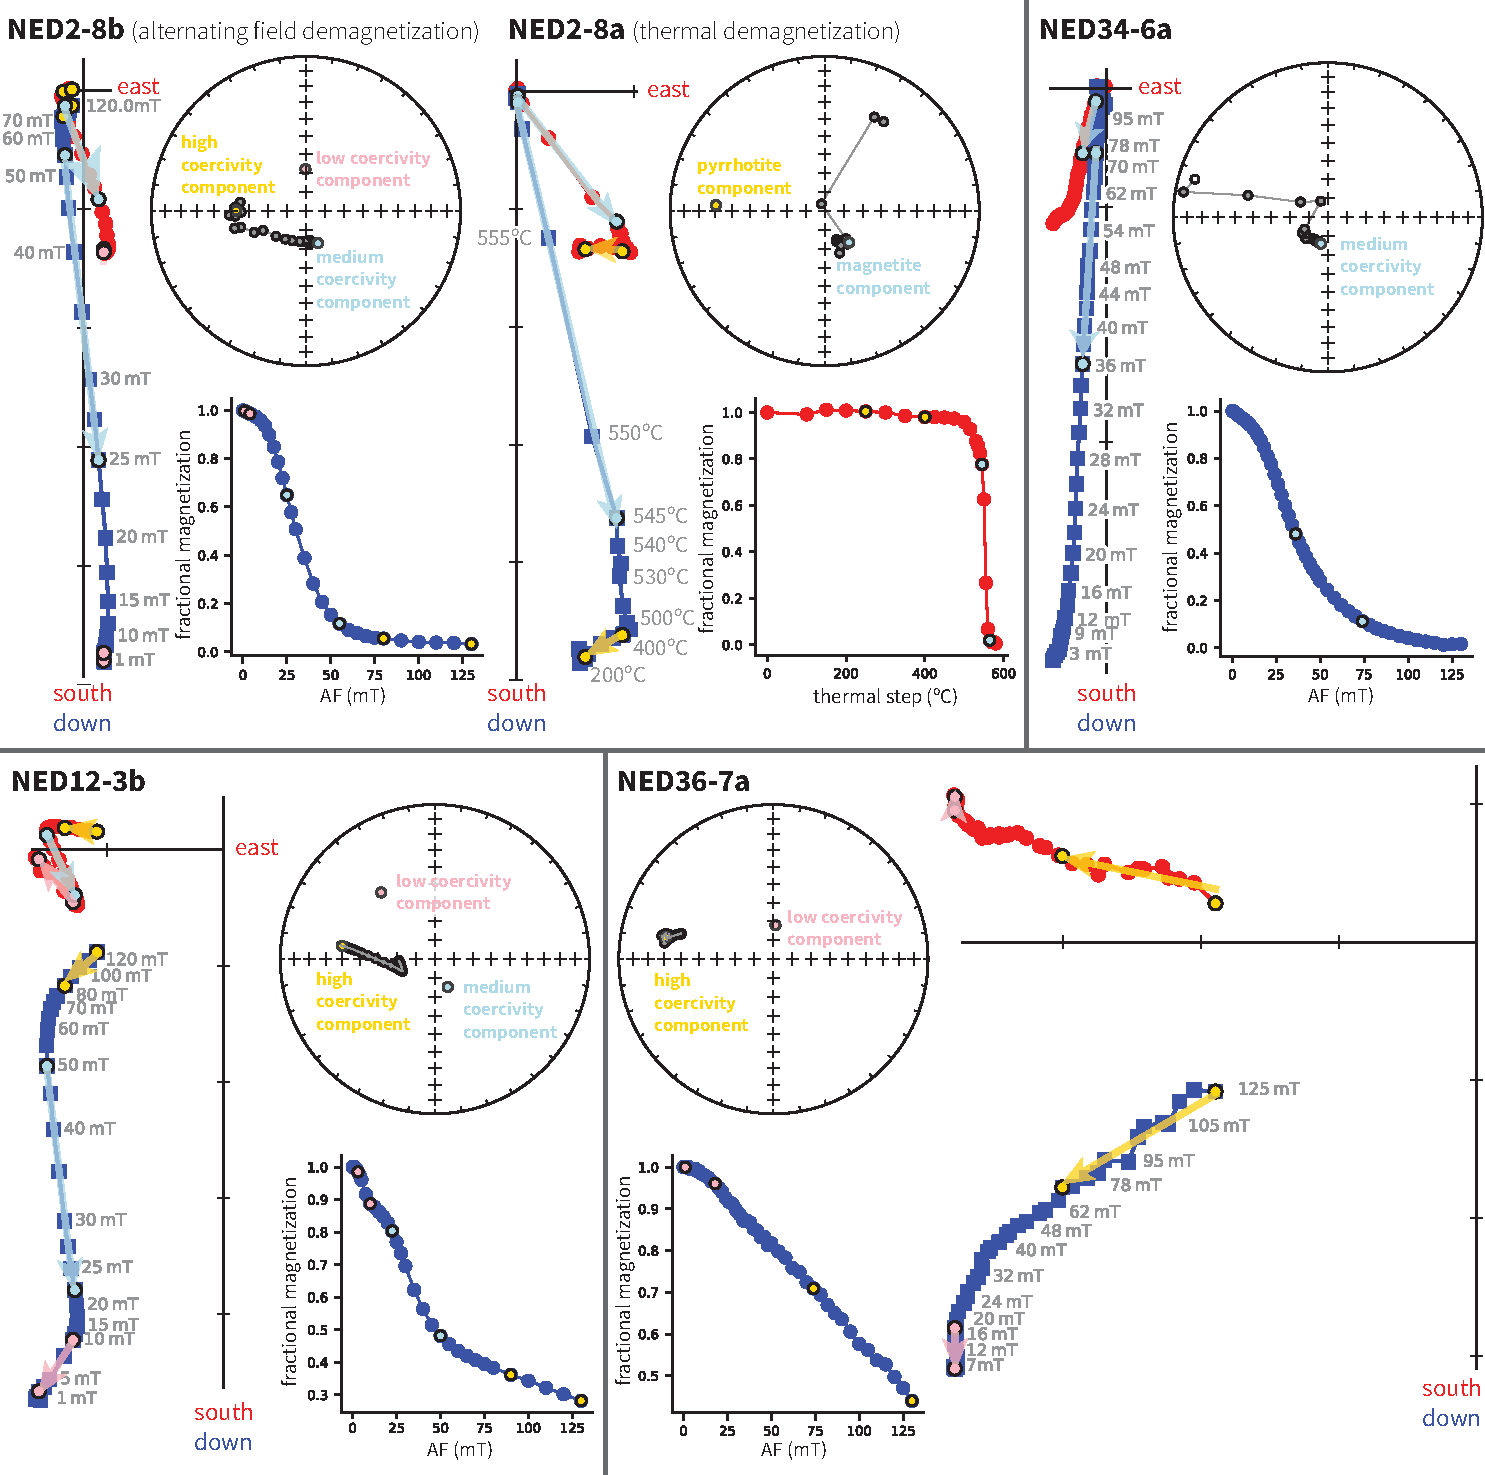
\includegraphics[width=\textwidth]{Figures/paleomag_data.pdf}
\caption{\setstretch{0.7}\small{Paleomagnetic data from ECMB diabase dikes are shown in geographic coordinates on vector component plots, measurement-level equal area plots and magnetization magnitude plots (developed using PmagPy; \citeA{Tauxe2016a}). Least-squares fits to the data are shown in colored arrows on the vector component plots, colored directions on the equal area plots, and as colored end-points on the magnetization magnitude plots (pink for low-coercivity; blue for medium-coercivity; yellow for high-coercivity). Specimens NED2-8a and NED2-8b are from the same core sample with them analyzed via thermal and alternating field (AF) demagnetization respectively. These data from sample NED2-8 reveal the steep medium-coercivity component to thermally unblock at temperatures characteristic of remanence held by magnetite and the high-coercivity component to thermally unblock at temperatures characteristic of remanence held by pyrrhotite. Specimen NED34-6a is dominated by the steep medium-coercivity component. The medium-coercivity component is well resolved in specimen NED12-3b which also has a substantial high-coercivity component. The high-coercivity component dominates the remanence of specimen NED36-7a such that no medium-coercivity component can be resolved.}}
\label{fig:example_pmag}
\end{figure}

Typical behaviors of sample remanence during demagnetization are illustrated for representative specimens in Figure \ref{fig:example_pmag}. AF demagnetization data typically reveal three components: a small low-coercivity component approximately aligned with Earth's present local field in the study region that was typically removed below 10 mT; a medium-coercivity component that is steep and was dominantly removed between 10 and 60 mT; and a high-coercivity component that was subsequently removed incompletely as demagnetization progressed to 130 mT. These components are present to varying degrees within individual specimens (Fig. \ref{fig:example_pmag}).

Sister specimens from the NED2 site underwent thermal and AF demagnetization which provides additional insight into the carriers of the components through comparison of the thermal and AF demagnetization spectra (Fig. \ref{fig:example_pmag}). These data reveal that the low-coercivity component direction is removed at the lowest unblocking temperatures up to 150\textdegree C. This behavior, as well as the typical direction, is most consistent with the component being acquired as a viscous overprint acquired in Earth's geomagnetic field. The direction of the high-coercivity component direction is removed through thermal demagnetization between 250\textdegree C and 350\textdegree C ---consistent with it being held by pyrrhotite. The direction of this high-coercivity component is aligned with the direction of magnetite-held remanence within a northwest-trending dike in the region (discussed in more detail below) --- a direction consistent with the position of Laurentia during the time period of \textit{ca.} 1095 Ma Midcontinent Rift magmatism \cite{Swanson-Hysell2020a}. We interpret this high-coercivity component, whose presence is variable in ECMB dikes, to have formed through hydrothermal activity associated with Midcontinent Rift magmatism such as that represented by the emplacement of the northwest-trending dike.  

In some specimens, the low-coercivity component is much larger and has a direction that is distinct from the present local field. It is likely that these samples acquired an isothermal remanent magnetization associated with quarrying operations. This behavior can be prevalent throughout a site or can be present in just some samples from a given site. In many cases, these low-coercivity overprints can be removed through AF demagnetization and medium-coercivity/high-coercivity components can be subsequently isolated. However, in some instances these large and dominantly low-coercivity overprints dominant much of the coercivity spectra preventing the isolation of other components.

The medium-coercivity component direction is dominantly removed between 515\textdegree C and 565\textdegree C consistent with it being held by low-Ti titanomagnetite. We interpret this component to be a primary thermal remanence acquired at the time of dike emplacement as part of the East Central Minnesota Batholith ca. 1779 Ma. This interpretation gains support from the rock magnetic data, an inverse baked contact test, and thermochronology data that support a mild thermal history that are discussed in more detail below. 

A Magnetic Properties Measurement System (MPMS) at the Institute for Rock Magnetism was used to conduct low-temperature remanence experiments. In the field-cooled (FC) experiments shown in Figure \ref{fig:MPMS_data}, the magnetization was measured upon warming following the specimen having cooled in an applied field of 2.5 T to 10 K. In the zero field-cooled (ZFC) experiment, a low-temperature saturation isothermal remanence (LTSIRM) of 2.5 T was applied at 10 K after the specimen cooled in a (near-)zero field. In the room-temperature saturation isothermal remanence (RTSIRM) experiment, the sample was pulsed with a 2.5 T field at room temperature and then cooled to 10 K and warmed back to room temperature in a (near-)zero field. These experiments reveal that sister specimens to paleomagnetic specimens whose remanence is dominated by the medium-coercivity component without an appreciable high-coercivity component have strong expressions of the $\sim$120 K Verwey transition as expected for a ferromagnetic mineralogy of well-preserved low-Ti titanomagnetite (NED34-6c Fig. \ref{fig:MPMS_data}). In contrast, specimens from samples that have a larger contribution of the high-coercivity component have weaker saturation magnetization, minor expression of the Verwey transition, and the presence of monoclinic pyrrhotite as evidenced through the $\sim$30 K Besnus transition (NED36-8c in Fig. \ref{fig:MPMS_data}). Samples with a more minor contribution of the high-coercivity component superimposed on the medium-coercivity component have intermediate behavior with a minor expression of the Besnus transition and a more prominent Verwey transition (NED2-8c in Fig. \ref{fig:MPMS_data}). These results support the interpretation that the medium-coercivity component is held by primary unaltered (titano)magnetite and that the high-coercivity component is the result of subsequent alteration that resulted in degradation of magnetite and pyrrhotite formation.

\begin{figure}[!ht]
\noindent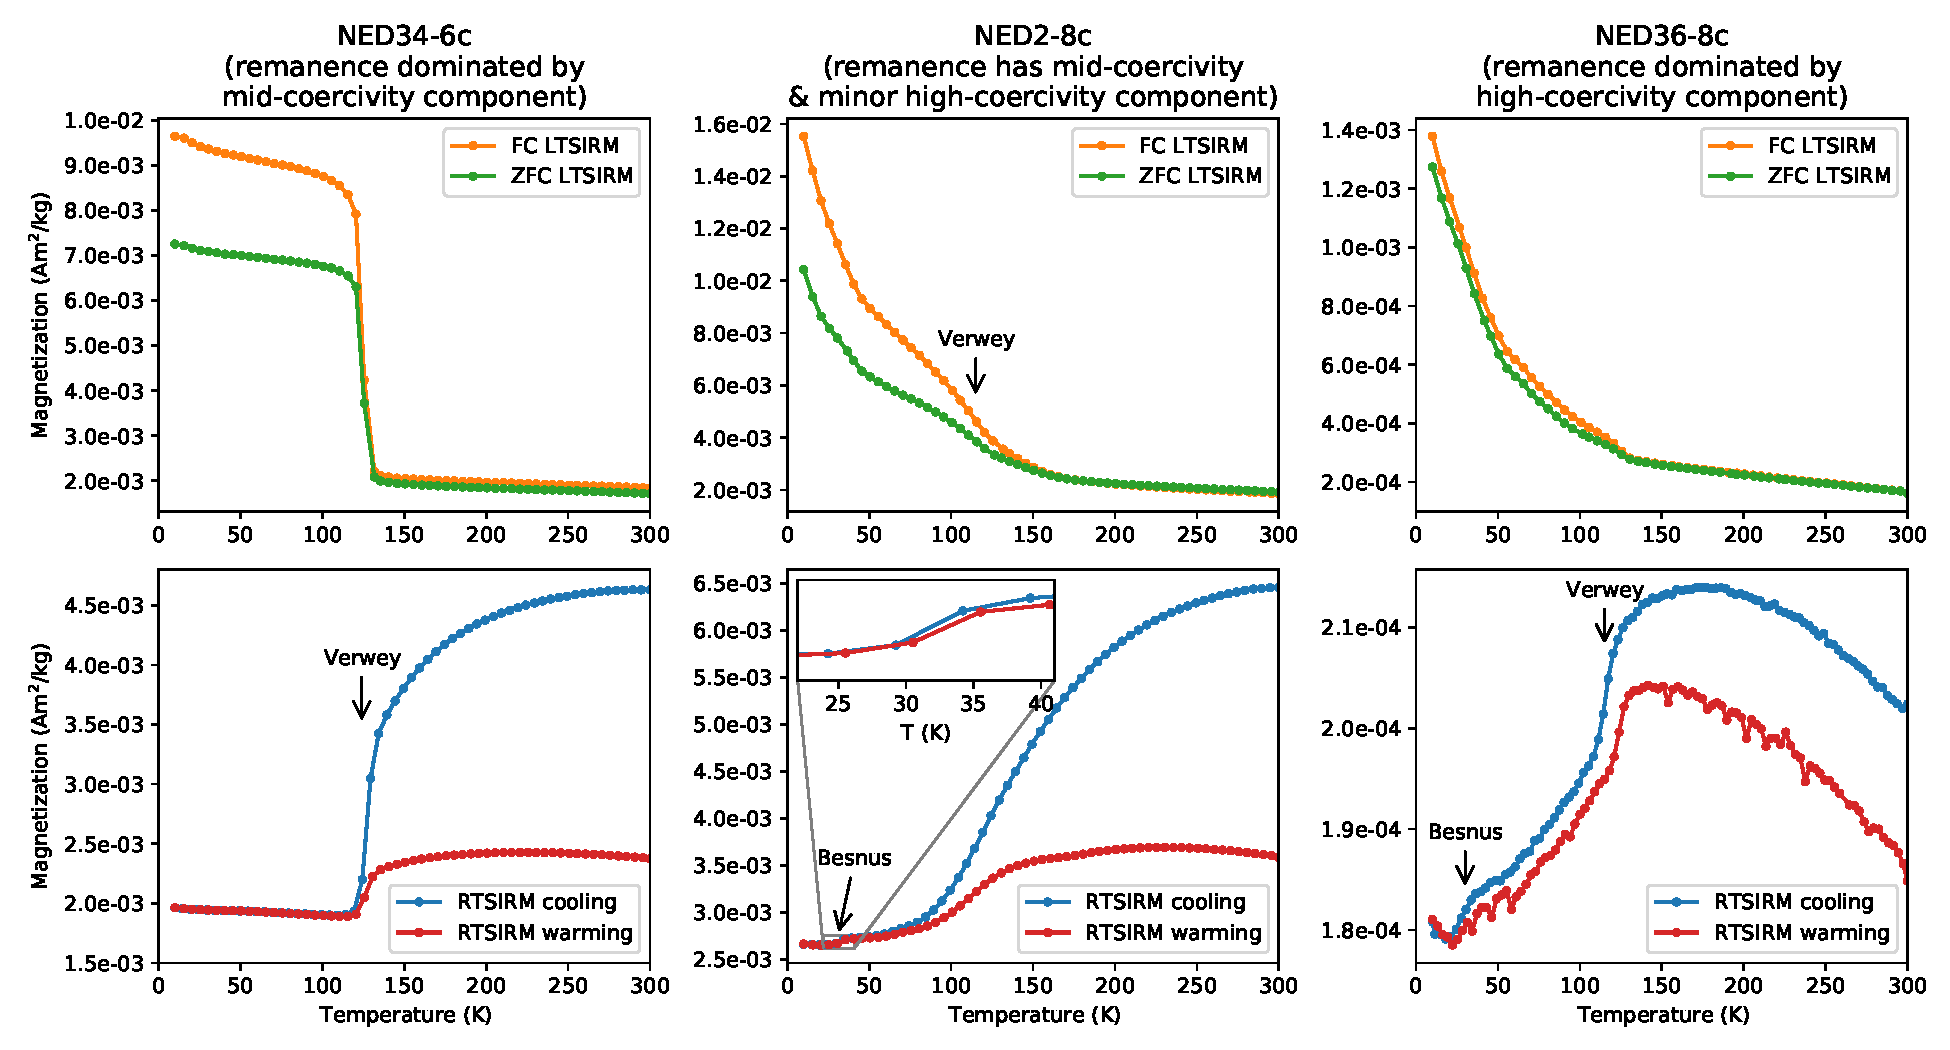
\includegraphics[width=\textwidth]{Figures/MPMS_data.pdf}
\caption{\setstretch{0.7}\small{Example results from low-temperature remanence experiments. The specimen from a sample whose natural remanence is dominated by the medium-coercivity component (NED34-6c) has behavior dominated by magnetite as evidenced through the response across the Verwey transition. The specimen from a sample whose natural remanence is dominated by the high-coercivity component (NED36-8c) has weaker magnetization, a relatively minor expression of the Verwey transition, and a Besnus transition that indicates the presence of monoclinic pyrrhotite. The specimen whose natural remanence has a well-resolved medium-coercivity component with a minor high-coercivity component (NED2-8c) has intermediate behavior with a Verwey transition that is not as suppressed as in NED36-8c with a minor, but resolvable Besnus transition (see inset). FC: field cooled; ZFC: zero-field cooled; LTSIRM: low-temperature saturation isothermal remanence magnetization; RTSIRM: room-temperature saturation isothermal remanence magnetization.}}
\label{fig:MPMS_data}
\end{figure}

One northwest-trending dike was exposed and sampled within the study region as site NWD1. The magnetization direction of this dike indicates that it is associated with the main stage of the Midcontinent Rift (ca. 1096 Ma) as it has a normal polarity and an inclination consistent with that time interval of Midcontinent Rift volcanism \cite{Swanson-Hysell2019a, Swanson-Hysell2020a}. The dike cross-cuts one of the northeast-trending dikes allowing for a baked contact test (Fig. \ref{fig:baked_contact}). The baked contact test is positive with a distinct direction in the northeast-trending dike (corresponding to the remanence direction seen throughout the northeast-trending dikes of the ECMB) with the magnetite remanence of the northeast-trending dike becoming progressively overprinted by the northwest-trending dike up the contact with it (Fig. \ref{fig:baked_contact}). This positive baked contact test indicates that the northeast-trending ECMB dikes have not been overprinted since the northwest-trending dike was emplaced (ca. 1095 Ma). This positive baked contact test for the northwest-trending dike constitutes what is referred to as a positive ``inverse'' baked contact test for the northeast-trending dike remanence --- it constrains the remanence to be more ancient than the ca. 1.1 Ga Mesoproterozoic northwest-trending dike, but does not provide a constraint back to the Paleoproterozoic time of dike emplacement. Given that the host rocks for the northeast-trending dikes are of a very similar age of the dikes themselves there is not the possibility of a Paleoproterozoic baked contact test and, in contrast to the dikes, stable remanence directions were not recovered from sites in the ECMB granite. 

The high-coercivity remanence direction held by pyrrhotite in some of the northeast-trending dikes is aligned with the remanence direction of the northwest-trending dike. While the thermal effect of the northwest-trending dike was limited to a few meters on either side of it as evidenced through the baked contact test, there was more widespread hydrothermal alteration associated with Midcontinent Rift magmatic activity that led to the formation of pyrrhotite. In the majority of the northeast-trending dikes, the original magnetite is well-preserved (as in NED34 of Figs. \ref{fig:example_pmag} and \ref{fig:MPMS_data}) while others experienced variable magnetite alteration and the formation of secondary pyrrhotite. These components can be separated through progressive demagnetization enabling the thermal remanent magnetization held by magnetite to be used to calculate a paleomagnetic pole.

\begin{figure}[!ht]
\noindent\includegraphics[width=\textwidth]{Figures/baked_contact.pdf}
\caption{\setstretch{0.7}\small{Results from a positive baked contact test where a northwest-trending dike (site NWD1) cross-cuts a northeast-trending dike (site NED17). The NWD1 dike has a direction indicating that it formed during the ca. 1095 Ma main stage of rift volcanism. Close to the NWD1 dike the NED17 is nearly full overprinted (NED17-1a). Further from NWD1 there are partial thermal overprints (NED17-7a) and that are then not resolvable $>$7 meters from the cross-cutting dike (NED17-11a).}}
\label{fig:baked_contact}
\end{figure}

The site mean directions determined from the magnetite remanence component can be used to calculate a mean paleomagnetic pole for the ECMB diabase dikes that utilizes data from 22 dikes (pole longitude: 265.8; pole latitude: 23.4; A$_{95}$: 6.2; Fig. \ref{fig:site_means}). In a massive host rock such as the ECMB plutons without preferential bedding or foliation, it is expected that lithospheric stresses will lead to the emplacement of near vertical dikes. Dike plane orientations were measured on each dike for which there was sufficient three-dimensional exposure. Multiple measurements were made for each dike to constrain their orientation. The mean strike calculated from 17 dike orientations is 067\textdegree and the mean dip is 88\textdegree. The $\alpha_{95}$ uncertainty associated with the Fisher mean for the poles to these dike orientation planes is 4.7\textdegree\ which means that the overall orientation of the planes is statistically indistinguishable from vertical. Due to this verticality, we interpret the exhumation of the ECMB plutons to have not resulted in appreciable tilting and do not apply a tilt correction to the paleomagnetic data.

\begin{figure}[!ht]
\noindent\includegraphics[width=\textwidth]{Figures/site_directions_pole.pdf}
\caption{\setstretch{0.7}\small{A) Site mean directions for the magnetite remanence of the northeast-trending (NED) ECMB diabase dikes with $\alpha_{95}<8$\textdegree. B) Virtual geomagnetic poles (VGPs) calculated from these site means and the overall mean paleomagnetic pole for the ECMB dikes. C) Comparison between the new ECMB paleomagnetic pole and other ca. 1780 to 1750 Ma poles for Laurentia. D) Comparison between 1780 to 1750 Ma poles for Laurentia and Baltica (Fennoscandia craton) without and with the rotation of Baltica in the NENA configuration.}}
\label{fig:site_means}
\end{figure}

\section*{Geochronology Methods and Results}

The field relationships show the diabase dikes to be younger than the Rockville granite, Reformatory granodiorite and the St. Cloud granite which they pervasively intrude and to be older than the Richmond granite in which they are absent. \cite{Holm2005a} developed U-Pb dates calculated as concordia intercept dates from these intrusive units. The dates reported by \cite{Holm2005a} for granites intruded by the dikes are 1783 $\pm$ 11 Ma for the Reformatory granodiorite, 1780 $\pm$ 7 Ma for the Rockville granite and 1779 $\pm$ 5 Ma for the St. Cloud granite. The younger cross-cutting Richmond granite has a date of 1772 $\pm$ 3 Ma \cite{Holm2005a}. An age of 1774 $\pm$ 7 Ma for one of the quartz-feldspar porphyry dikes developed by \cite{Holm2005a} is consistent with this interpretation of these dikes being older than the Richmond granite (and younger than the granites they intrude). While the dates published in \citeA{Holm2005a} are valuable constraints, they are of lower precision than what is possible with modern analytical approaches and therefore lead to overlapping uncertainties. Higher precision constraints can test the field relationship interpretations and provide more confidence in the overall age constraints.

\begin{figure}[!ht]
\centering
\noindent\includegraphics[width=\textwidth]{Figures/ECMB_dates.pdf}
\caption{\setstretch{0.7}\small{U-Pb dates for ECMB samples. Weighted means are calculated from individual zircon dates. The NED diabase dikes intrude the St. Cloud granite such that the ECMB6 weighted mean date of 1781.44$\pm$0.51 Ma is a maximum age. The quartz-feldspar porphry dikes (one of which was sampled as QP1) also intrude the St. Cloud Granite and are parallel to the NED diabase dikes. Neither the quartz-porphry dikes nor the diabase dikes intrude the younger cross-cutting Richmond granite such that the ECMB4 weighted mean date of 1776.49$\pm$0.49 Ma provides a minimum age for the dikes.}}
\label{fig:U_Pb_dates}
\end{figure}

To further constrain the age of the northeast-trending diabase dikes, we developed new isotope dilution-thermal ionization mass spectrometry (ID-TIMS) U-Pb zircon dates from the St. Cloud granite that host the dikes (sample ECMB6), the Richmond granite from which the dikes are absent (sample ECMB4), and from a northeast-trending quartz-feldspar porphyry dike (sample QP1) that is likely coeval with the diabase dikea . Zircon crystals were chemically abraded prior to analysis of single zircon grains by ID-TIMS at the Boise State Isotope Geology Laboratory (detailed geochronology methods are provided in the Supporting Information). Weighted mean dates were calculated from multiple single zircon dates (Fig. \ref{fig:U_Pb_dates}; Table \ref{tab:geochron}). While chemical abrasion served to reduce Pb-loss and resulted in concordant analyses, some grains have persistent Pb-loss and are discordant (Fig. S1). As a result, we calculate weighted mean  $^{207}$Pb/$^{206}$Pb dates rather than $^{206}$Pb/$^{238}$U dates (Fig. \ref{fig:U_Pb_dates}). These $^{207}$Pb/$^{206}$Pb dates are 1781.44$\pm$0.51 Ma (2$\sigma$ analytical uncertainty) for the St. Cloud granite and 1776.76$\pm$0.49 Ma for the Richmond granite (Fig. \ref{fig:U_Pb_dates}). The date for the sampled quartz-feldspar porphyry dike of 1780.78$\pm$0.45 Ma is between these two dates as expected on the basis of field relationships. Taking into account the analytical uncertainty on the dates, the diabase dikes are younger than 1782 Ma (age of the St. Cloud Granite) and older than 1776 Ma (age of the Richmond Granite). We can succinctly state the age of the dikes as being 1779 $\pm$ 3 Ma. 

\begin{table}[h!]
\footnotesize
\caption{Summary of ID-TIMS $^{207}$Pb/$^{206}$Pb East Central Minnesota Batholith dates}
\begin{tabular}{p{1 cm}p{2.4 cm}p{1.8 cm}ccccc}
\hline
Sample & Unit & Latitude & $^{207}$Pb/$^{206}$Pb & \multicolumn{2}{c}{Uncertainty (2$\sigma$)} & MSWD & n/N \\
 &  & Longitude & date (Ma) & X & Z & & \\
\hline
ECMB6 & St. Cloud granite & 45.53396$^{\circ}$ N 94.23187$^{\circ}$ W & 1781.44 & 0.51 & 2.4 & 1.24 & 8/8 \\
%\hline
QP1 & quartz-feldspar porphyry dike & 45.53481$^{\circ}$ N 94.25811$^{\circ}$ W & 1780.78 & 0.45 & 2.4 & 0.53 & 8/8 \\
%\hline
ECMB4 & Richmond granite & 45.44343$^{\circ}$ N 94.48360$^{\circ}$ W & 1776.76 & 0.49 & 2.4 & 1.15 & 7/8 \\
\hline
\end{tabular}\\
%\begin{tablenotes}[para,flushleft]
Notes: X is 2$\sigma$ analytical uncertainty; Z is 2$\sigma$ uncertainty including decay constant uncertainty. This Z uncertainty needs to be utilized when comparing to dates using other decay systems (e.g., $^{40}$Ar/$^{39}$Ar, $^{187}$Re-$^{187}$Os); MSWD is the mean squared weighted deviation; n is the number of individual zircon dates included in the calculated sample mean date; N is the number of individual zircons analyzed for the sample.
%\end{tablenotes}
\label{tab:geochron}
\end{table}

\section*{Thermochronology Methods and Results}

While the U-Pb zircon dates constrain the crystallization ages of the ECMB intrusions, additional insight into the thermal history of the batholith can help to interpret the paleomagnetic data. As discussed below, existing Ar-Ar dates on hornblende and biotite from the ECMB provide valuable constraints in this regard. In this study, we also developed U-Pb apatite dates from three ECMB granites (ECMB1, the Isle Granite; ECMB3, the Rockville Granite; ECMB4, the Richmond Granite). In contrast to zircon for which the temperatures at which Pb will appreciably diffuse out of a crystal exceeds the liquidus of granite, the temperature window for closure of the U-Pb system in apatite is much lower ($\sim$ 520 to 430\textdegree C; \citeA{Smye2018a}). As a result, U-Pb dates of apatite serve as a thermochronometer at moderately high temperatures \cite{Chamberlain2001a, Schoene2007a, Chew2015a}. These temperatures are of particular relevance to the interpretation of the paleomagnetic data as they are lower than or correspond with the blocking temperature of low-titanium titanomagnetite. If a pluton was emplaced at depths where temperatures exceed the closure temperature of apatite or if it experienced prolonged reheating, the U-Pb apatite dates would be appreciably younger than the U-Pb zircon crystallization dates.

U-Pb data were developed from apatite grains separated from ECMB granites through laser ablation inductively coupled plasma mass spectrometry (LA-ICP-MS) at UC Santa Barbara. In contrast to zircon, apatite incorporates significant Pb at the time of crystallization. As a result of this elevated common Pb, U-Pb dates were determined through the calculation of Tera-Wasserburg concordia intercept dates where the upper intercept corresponds to the ratio of initial $\^{207}$Pb/$\^{206}$Pb and the lower intercept is the $\^{206}$Pb/$\^{238}$U date (following the method of \citeA{Ludwig1998a} as implemented in IsoPlotR \citeA{Vermeesch2018a}; Fig. S2). Sample ECMB1 is from the Isle Granite which has a U-Pb zircon date of 1779 $\pm$ 26 Ma. The U-Pb apatite date is  1800.3 $\pm$ 16.7/65.2 Ma where the first uncertainty is the 2$\sigma$ analytical uncertainty and the second uncertainty is 95$\%$ confidence interval for the date that incorporates overdispersion. This U-Pb apatite date is therefore indistinguishable from the U-Pb crystallization date.  Sample ECMB 

%Additional insight
%
%
%{\color{red}{John and Francisco, can you send along methods text that can be incorporated here?}}
%
%
%
%U-Pb apatite date 
%
%
%
%In order to constrain the thermal history of the East Central Minnesota Batholith U/Pb dates were developed from  {\color{red}{Brenhin and David, can you send along methods text that can be incorporated here?}}
%
%



\section*{Discussion}

\subsection*{Thermal history of the ECMB and a primary interpretation of the ECMB dike pole}

Prior to the emplacement of the ECMB, Paleoproterozoic metasedimentary host rocks were metamorphosed to amphibolite facies during the Penokean orogeny \cite{Holm1990a}. Emplacement of the ECMB has been hypothesized to be post-orogenic and associated with an interval of extensional collapse of the orogen \cite{Holm1998a, Boerboom2000a}. The Al-in-hornblende igneous barometer was applied to the St. Cloud and Isle granites of the ECMB by \cite{Holm1998a}. This barometer has varying published calibrations. Applying the pressure calibration of \cite{Mutch2016a} and assuming a 2.7 g/cm$^{3}$ overburden gives an estimated emplacement depth of $\sim$10.4 $\pm$ 1.7 km for the Isle granite and $\sim$13.4 $\pm$ 2.1 km for the St. Cloud granite. The calibration of \cite{Ague1997a} leads to slightly higher calculated pressures implying depths that are $\sim$2.5 km deeper. 

\begin{figure}[!ht]
\centering
\noindent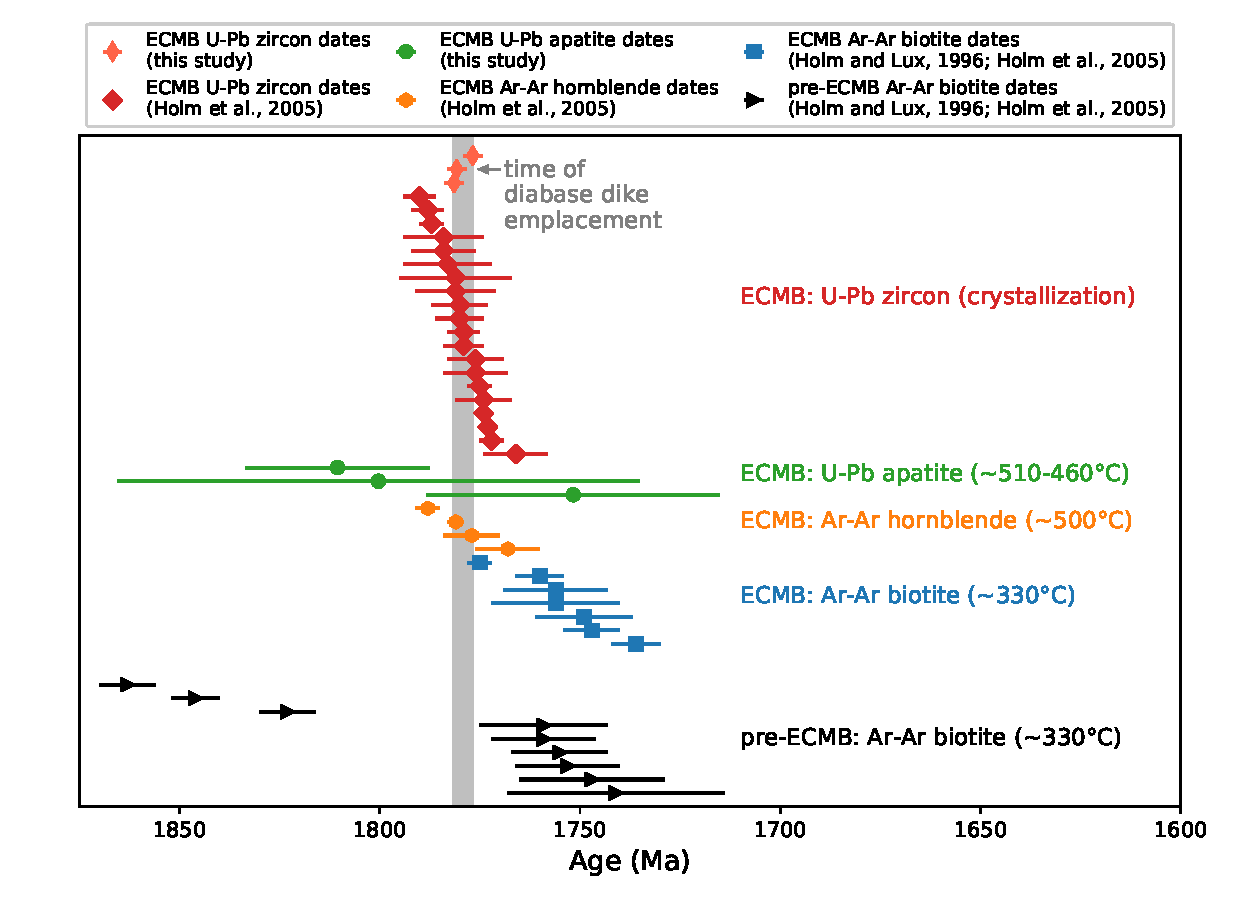
\includegraphics[width=\textwidth]{Figures/ECMB_dates_thermochron}
\caption{\setstretch{0.7}\small{Summary of U-Pb zircon dates, U-Pb apatite dates, Ar-Ar hornblende, and Ar-Ar biotite dates from the East Central Minnesota batholith. That the U-Pb apatite and Ar-Ar hornblende dates are indistinguishable from the U-Pb zircon crystallization dates indicating that the plutons were emplaced at upper crustal levels.}}
\label{fig:U_Pb_dates}
\end{figure}

Thermochronology data give additional insight in this regard. Both the Ar-Ar hornblende dates published by \citeA{Holm2005a} and the U-Pb apatite dates developed in this study developed from ECMB lithologies are indistinguishable from the crystallization ages of the intrusives. The closure temperature for Ar in hornblende is $\sim$580 to 490\textdegree C \cite{Harrison1982a}. The closure of the U-Pb system in apatite is $\sim$ 520 to 430\textdegree C \cite{Smye2018a}. The consistency between the U-Pb zircon crystallization and the U-Pb apatite and Ar-Ar hornblende cooling dates indicates that the present-day erosion level of the ECMB was at a shallow enough depth that the temperatures were lower than these closure temperatures at the time of emplacement of the plutons. Geothermal gradients in continental arc settings are typically between 25 to 45\textdegree C/km -- potentially higher at 1.8 Ga \cite{Rothstein2003a}. Taking a geothermal gradient of 30\textdegree C/km and the closure temperature constraints indicates that the plutons were emplaced at 15 km or shallower in the continental lithosphere. These relatively shallow crustal depths are consistent with the Al-in-hornblende paleobarometry estimates. Ar-Ar biotite dates provide insight to even lower temperatures as the system blocks at $\sim$330\textdegree C \cite{Grove2001a}. The ECMB Ar-Ar biotite dates range from overlapping the crystallization dates to being younger by a few tens of millions of years. Ar-Ar biotite dates from older host lithologies to the ECMB are consistently older than the age of the batholith itself which suggests that the these host rocks and the batholith were emplaced at crustal levels where the temperature was $<$330\textdegree C and therefore at the upper depth range estimates from the Al-in-hornblende barometry ($\sim$ 10 km). 

The magnetization used to develop the paleomagnetic pole comes from remanence held by low-titanium magnetite that dominantly unblocks between 540 to 560\textdegree C (Figs. \ref{fig:example_pmag} and \ref{fig:baked_contact}). The thermochronology results constrain thermal history of the rocks to have cooled through the blocking temperatures at the time that the dikes were emplaced within the batholith and to not have experience reheating that would have perturbed the thermochronometers. These data support an interpretation that the magnetite remanence within the ECMB dikes is a primary thermal remanent magnetization 

Following the emplacement of the ECMB, there are few tectonothermal events in the region with the potential to have modified the magnetization of the magnetite within the ECMB diabase dikes. This mild subsequent history is supported by the U-Pb apatite, Ar-Ar hornblende and Ar-Ar biotite thermochronometers all giving ages from the time of initial crystallization. Subsequent Paleoproterozoic Yavapai and Mazatzal accretion occurred to the southeast of the Spirit Lake Tectonic zone on the other side of the Minnesota River Valley promontory and Marshfield terrane (Fig. \ref{fig:Laurentia_map}, \citeA{Holm2007b}). In contrast to the northeast-trending dikes in the ECMB, northeast-trending dikes in Wisconsin within ca. 1770 Ma plutons were metamorphosed to amphibolite facies associated with such accretionary orogenesis \cite{Holm1998b}. Mazatzal deformation and metamorphism occurred ca. 1650 to ��1630 Ma within the juvenile accreted island arc of the Wisconsin magmatic terrane and led to compressional deformation in the Paleoproterozoic Baraboo quartzite \cite{Holm1998c}. The region of the ECMB was not affected by this tectonothermal event nor was the region of the flat-lying Sioux Quartzite further to the southwest (Fig.\ref{fig:Laurentia_map}, \citeA{Holm2005a}). \citeA{Holm2005a} propose that the voluminous ECMB batholith stablized the continental lithosphere and prevented the region from being modified during subsequent collisions along the margin.

Yavapai and Mazatzal terranes were intruded by ca. 1470 to 1430 Ma granites of the Eastern Granite Rhyolite Province and there is a major pluton within accreted Penokean rocks in northern Wisconsin (the ca. 1470 Ma Wolf River batholith; \cite{Dewane2007a}). However, the thermal effects of the Wolf River batholith ($\sim$370 km east of the study area) were limited to a 10-15 km wide contact zone surrounding the intrusion \cite{Holm2019a}. 

%Could discuss evidence for rapid exhumation as discussed in Holm 
%The deposition of the fluvial sandstone of the Sioux Quartzite atop post-Penokean intrusions 
%Is the Siouz Quartzite flat-lying, what are the best constraints on its age?

The one major subsequent tectonothermal event in the region for which there is evidence in the ECMB is the development of the Midcontinent Rift that initiated ca. 1109 Ma and in which magmatic activity continued to ca. 1084 Ma \cite{Fairchild2017a, Swanson-Hysell2019a}. While the main rift axis can be inferred from aeromagnetic anomaly data to be located $\sim$75 km southeast of the study region (Fig. \ref{fig:Laurentia_map}), the studied northwest-trending dike has a magnetization direction that implies that it was emplaced during Midcontinent Rift development (Fig. \ref{fig:baked_contact}). The baked contact test between that dike (NWD1) and the northeast-trending dike that it cross-cuts (NED17), indicates that the thermal effect of the dike emplacement and the Midcontinent Rift in general was localized within the immediate vicinity of that dike (a few meters; Fig. \ref{fig:baked_contact}). However, this Midcontinent Rift magmatic activity did result in local hydrothermal alteration as evidenced through a magnetic overprint held by pyrrhotite that is variably present through the ECMB dikes and is in the same direction as the magnetization of the northwest-trending dike. While in some sites, this alteration obscured the primary thermal remanence held by magnetite, in the majority of sites the magnetite remanence direction can be well-resolved. As a result, the paleomagnetic directions used to calculate the paleomagnetic pole shown in Figure \ref{fig:site_means} are held by (titano)magnetite that recorded a thermal remanence magnetization upon cooling of the diabase dikes. Evidence for late Mesoproterozoic hydrothermal alteration of the dikes provides an explanation for Ar-Ar data reported in \cite{Boerboom2000a}. Ar-Ar data developed from two northeast-trending diabase dikes did not yield a plateau age, but give whole rock total gas dates that are late Mesoproterozoic in age. An interpretation that these whole rock total gas ages correspond with the age of emplacement is difficult to reconcile with the cogenetic relationship between the diabase dikes and the quartz-feldspar porphyry dikes. K-Ar whole-rock ages of 1570 to 1280 Ma from the dikes reported in \cite{Hanson1968a} and discussed in \cite{Horan1987a} are attributed to partial resetting. The magnetic evidence for fluid flow and formation of pyrrhotite ca. 1095 Ma supports this hypothesis put forward by both \cite{Horan1987a}, as well as by \cite{Boerboom2000a}, that there was Mesoproterozoic disruption of the K-Ar isotopic system in the dikes such that the Mesoproterozoic Ar-Ar dates are the result of alteration of dikes which are Paleoproterozoic in age. This interpretation based on the field relationships that the north-east trending diabase dikes are comagmatic with ECMB granites is consistent with whole rock Pb isotope data that reveal very similar arrays implying a roughly 1.8 Ga isochron age for both lithologies \cite{Horan1987a}. 

%The Section 28 Granite from the Minnesota River Valley was precisely dated at ~1781 Ma and also displays impressive comingling textures with mafic enclaves (see fig. 4 in that paper and unit descriptions). Perhaps the occurrence of this similar lithology and date should also be mentioned in the Discussion.

The ECMB, including the comagmatic dikes of this study, were emplaced in the upper crust and would have acquired their magnetization at the time of emplacement. The lack of significant thermal events that could have reset the magnetite magnetization is indicated by the geologic setting, the thermochronology data, and the positive inverse baked contact test. We therefore interpret the ECMB diabase pole as a high-quality constraint on the paleogeographic position of Laurentia ca. 1779$\pm$3 Ma.

\begin{table}[h!]
\footnotesize
\caption{Summary of paleomagnetic poles}
\begin{tabular}{|p{3 cm}|r|r|r|r|r|r|r|r|}
\hline
unit name & age (Ma) &pole lon (\textdegree) & pole lat (\textdegree) & A$_{95}$ & K & R & N & reference \\
\hline
ECMB diabase dikes \textit{southern Superior province} & 1779 $\pm$ 3 Ma & 265.8 & 23.4 &  6.2 & 26.0 & 21.2 &  22 & this study \\
\hline
Jan Lake Granite \textit{trans-Hudson orogen} & 1758 $\pm$ 1 Ma &  &  &  6.2 &  &  &  & \cite{Gala1995a} \\
\hline
\end{tabular}
\begin{tablenotes}
Notes: pole lon--longitude of paleomagnetic pole; pole lat--latitude of paleomagnetic pole; A$_{95}$--confidence limit of pole mean degrees; K--Fisher precision parameter; R--resultant vector length; N--number of dike site mean virtual geomagnetic poles used to calculate the mean pole.
\end{tablenotes}
\label{tab:poles}
\end{table}

\subsection*{The paleogeography of Laurentia}

While abundant paleomagnetic data have been developed from rocks within the Trans-Hudson orogen, both the primary nature of remanence directions as well as the age of remanence acquisition has been challenging to establish. As a result, few poles from this interval of Laurentia's final amalgamation have been included in curated pole compilations such as that compiled by the Nordic paleogeography workshops \cite{Evans2021a}. The poles that have been included in the \citeA{Evans2021a} compilation are that from the ca. 1766 Ma Deschambault Pegmatites, the ca. 1758 Ma Jan Lake Granite and the ca. 1740 Ma Cleaver Dykes. The best constrained of these poles is that from the post-orogenic 1740 $\pm$ 5 Ma Ma Cleaver Dykes of the Great Bear Magmatic Arc to the west of the Slave Province \cite{Irving2004a}. The age of these dikes is constrained by a U-Pb baddeleyite date and there is a positive baked contact test supporting the interpretation that the pole is primary. As can be seen in Figure \ref{fig:pole_comparison}, the position of this ca. 1740 Ma pole for Laurentia is similar to the new pole for the ca. 1780 Ma ECMB diabase dikes. The poles have distinct mean directions (as determined through Watson and bootstrap common mean tests), but are within 11\textdegree\ of one another. This similarity indicates a similar position of Laurentia at ca. 1780 and ca. 1740 Ma. A less robust pole comes from the post-orogenic Jan Lake Granite from the Trans-Hudson orogen in southeast Saskatchewan developed in \citeA{Gala1995a}. A U-Pb zircon date of 1758 $\pm$ 1 Ma for this granite was reported in \citeA{Bickford2005a}. Directional data from the Jan Lake Granite falls into two groups. Based on the demagnetization behavior, \cite{Irving2004a} interpreted the `A' grouping to be a TRM acquired at the time of the emplacement of the intrusion ca. 1758 Ma.  The ECMB dikes pole shares a common mean with this Jan Lake Granite pole with overlapping A$_{95}$ confidence circles. This result is consistent with the both the Jan Lake Granite and ECMB being post-orogenic magmatic events that occurred following the amalgamation of Laurentia. This similarity suggests that despite the large uncertainty on the Jan Lake Granite pole and the ambiguity resulting from multiple direction groups that the pole does constrain the position of Laurentia ca. 1758 Ma.

A pole that does not hold up to such comparative scrutiny is that developed for the Deschambault Pegmatites from within the Trans-Hudson orogen \cite{Symons2000a}. This pole has been interpreted to constrain the position of Laurentia ca. 1766 Ma --- an age based on U-Pb monazite and allanite dates of other pegmatites in the region. As noted in \cite{DAgrella-Filho2020a}, there are no field tests for this pole and the remanence directions from which it is calculated are quite close to the modern geomagnetic field. The direction of the Deschambault pole is far from the new ca. 1780 Ma ECMB dikes pole. In contrast, the similarity of pole position between the new ECMB dikes pole and the the ca. 1758 Ma Jan Lake Granite pole as well as the ca. 1740 Ma Cleaver dike pole supports that these poles, rather than the Deschambault Pegmatites pole, constrain Laurentia's position during this interval. The Deschambault Pegmatites pole should no longer be used for paleogeographic analysis. 

The Trans-Hudson orogeny is a major event in the formation of Laurentia resulting from the collision between the Superior province and the composite Slave+Rae+Hearne provinces \cite{Corrigan2009a}. A $^{206}$Pb/$^{238}$U date of 1854.2 $\pm$ 1.6 Ma from the base of a foredeep sedimentary succession on the northern margin of the East Superior province constrains Trans-Hudson orogenesis to have been ongoing and driving flexural subsidence at that time \cite{Hodgskiss2019a}. This timing of orogenesis is consistent with $^{207}$Pb/$^{206}$Pb dates of monazite within garnet of Trans-Hudson orogen ecologites for which a mean date of 1831 $\pm$ 5 Ma has been interpreted to record peak metamorphism \cite{Weller2017a}. A similar timing of ca. 1860 to 1820 Ma peak Trans-Hudson metamorphism resulting from collisional orogenesis has been interpreted from U-Pb zircon rim and monazite dates from the orogen in Baffin Island \cite{Skipton2016a}. With this context, it is not surprising the similar pole positions ca. 1785 to 1740 Ma should be obtained from the Superior Province (the new ECMB pole), the Trans-Hudson orogen (the Jan Lake Granite pole), and from provinces accreted to the Slave Province (the Cleaver dikes pole). Nevertheless, the overlap between these poles provides an independent test of the coherency of the Laurentia craton at that time. 

With the new ECMB pole, we can have higher confidence in paleogeographic reconstructions in the time just following the amalgamation of Archean provinces into a coherent Laurentia craton. These new data can be used to evaluate hypothesized connections between Laurentia and other cratons. One hypothesized connection of particular interest is that with Baltica. The two cratons have been hypothesized to share 

%For example, the new pole is consistent with NENA connection between Laurentia and Baltica being established prior to this time prior to the long-lived history of accretionary orogenesis along that joint margin.
%
%Salminen, J., Mertanen, S., Evans, D.A.D., Wang, Z., 2014b. Paleomagnetic and geochemical studies of the Mesoproterozoic Satakunta dyke swarms, Finland, with implications for a Northern Europe ? North America (NENA) connection within Nuna supercontinent. Precambrian Research 244, 170?191.
%
%Johanna's description of the Svecofennian orogen is as follows:
%"5.2.2.2 Crustal growth of Fennoscandia ? the Svecofennian orogen
%Paleoproterozoic 2.1 ? 1.8 Ga global orogenic events that reflect the assembly of supercontinent Nuna are recorded in Fennoscandia. The majority of the Paleoproterozoic crustal growth of Fennoscandia occurred during the Svecofennian orogen (Lahtinen et al., 2008) and different tectonic models have been presented for the  orogen (summaries in e.g. Bogdanova et al., 2015; Nironen, 2017). In one model, sediments and volcanic rocks were deposited in a wide marginal basin along an active continental margin of the Archean Karelian craton (Rutland et al., 2001, 2004; Williams et al., 2008). Modified models suggest that several island arcs were accreted along the single continental margin during continuous subduction (G�al and Gorbatschev, 1987; BABEL working group, 1990; Gorbatchev and Bogdanova, 1993; Bogdanova et al., 2015) or with separate periods of subduction and compression, leading to extensional and compressional cycles in the overriding plate (Hermansson et al., 2008; Saalmann et al., 2009; Nironen 2017).
%
%In an entirely different model the growth of Fennoscandia has been explained by several orogenic stages (Nironen, 1997; Lahtinen et al., 2005, 2009). According to Lahtinen et al. (2005, 2009) the composite Svecofennian orogen is a collage of 2.1 ? 2.0 Ga microcontinents and 2.02 ? 1.82 Ga island arcs accreted with the Karelian craton at 1.92 ? 1.79 Ga. This accretion of island arcs and microcontinents extended down to Trans-European suture zone in the southwest of Fennoscandia. A first accretion at 1.92 ? 1.87 Ga was followed by continental extension at 1.86 ? 1.84 Ga. Semi-simultaneously with the accretion in southwest Fennoscandia collided with Volgo-Sarmatia at 1.84 ? 1.79 Ga (Svecobaltic orogeny) in the east and after an orogenic collapse at 1.79 ? 1.77 Ga the crust stabilized. The collision between Fennoscandia and Volgo-Sarmatia also involved also the southeastern part of Fennoscandia, where the bedrock is primarily comprised of alternating NW-SE trending belt-shaped tectonic domains that were stacked in the collision (Bogdanova et al., 2015).
%"
%
%Her 2019 paper also cites all of these:
%(Salminen and Pesonen, 2007; Evans and Pisarevsky, 2008; Salminen et al., 2009; Lubnina et al., 2010; Pisarevsky and Bylund, 2010; Evans and Mitchell, 2011; Salminen et al., 2014b, 2015, 2017; Lubnina et al., 2017)
%
%Make a Baltica-Laurentia comparison figure in the NENA configuration.
%
%Euler parameters of Baltica to North America given in Evans2013b are (65.2, 218.1, –43.7)
%
%Check out the Sao Francisco pole and paleogeography discussion in
%DAgrella-Filho2020a





%Text here ===>>>

%%

%  Numbered lines in equations:
%  To add line numbers to lines in equations,
%  \begin{linenomath*}
%  \begin{equation}
%  \end{equation}
%  \end{linenomath*}



%% Enter Figures and Tables near as possible to where they are first mentioned:
%
% DO NOT USE \psfrag or \subfigure commands.
%
% Figure captions go below the figure.
% Table titles go above tables;  other caption information
%  should be placed in last line of the table, using
% \multicolumn2l{$^a$ This is a table note.}
%
%----------------
% EXAMPLE FIGURE
%
% \begin{figure}[h]
% \centering
% when using pdflatex, use pdf file:
% \includegraphics[natwidth=800px,natheight=600px]{figsamp.pdf}
%
% when using dvips, use .eps file:
% \includegraphics[natwidth=800px,natheight=600px]{figsamp.eps}
%
% \caption{Short caption}
% \label{figone}
%  \end{figure}
%
% We recommend that you provide the native width and height (natwidth, natheight) of your figures.
% Specifying native dimensions ensures that your figures are properly scaled
%
%
% ---------------
% EXAMPLE TABLE
%
% \begin{table}
% \caption{Time of the Transition Between Phase 1 and Phase 2$^{a}$}
% \centering
% \begin{tabular}{l c}
% \hline
%  Run  & Time (min)  \\
% \hline
%   $l1$  & 260   \\
%   $l2$  & 300   \\
%   $l3$  & 340   \\
%   $h1$  & 270   \\
%   $h2$  & 250   \\
%   $h3$  & 380   \\
%   $r1$  & 370   \\
%   $r2$  & 390   \\
% \hline
% \multicolumn{2}{l}{$^{a}$Footnote text here.}
% \end{tabular}
% \end{table}

%% SIDEWAYS FIGURE and TABLE
% AGU prefers the use of {sidewaystable} over {landscapetable} as it causes fewer problems.
%
% \begin{sidewaysfigure}
% \includegraphics[width=20pc]{figsamp}
% \caption{caption here}
% \label{newfig}
% \end{sidewaysfigure}
%
%  \begin{sidewaystable}
%  \caption{Caption here}
% \label{tab:signif_gap_clos}
%  \begin{tabular}{ccc}
% one&two&three\\
% four&five&six
%  \end{tabular}
%  \end{sidewaystable}

%% If using numbered lines, please surround equations with \begin{linenomath*}...\end{linenomath*}
%\begin{linenomath*}
%\begin{equation}
%y|{f} \sim g(m, \sigma),
%\end{equation}
%\end{linenomath*}

%%% End of body of article

%%%%%%%%%%%%%%%%%%%%%%%%%%%%%%%%
%% Optional Appendix goes here
%
% The \appendix command resets counters and redefines section heads
%
% After typing \appendix
%
%\section{Here Is Appendix Title}
% will show
% A: Here Is Appendix Title
%
%\appendix
%\section{Here is a sample appendix}

%%%%%%%%%%%%%%%%%%%%%%%%%%%%%%%%%%%%%%%%%%%%%%%%%%%%%%%%%%%%%%%%
%
% Optional Glossary, Notation or Acronym section goes here:
%
%%%%%%%%%%%%%%
% Glossary is only allowed in Reviews of Geophysics
%  \begin{glossary}
%  \term{Term}
%   Term Definition here
%  \term{Term}
%   Term Definition here
%  \term{Term}
%   Term Definition here
%  \end{glossary}

%
%%%%%%%%%%%%%%
% Acronyms
%   \begin{acronyms}
%   \acro{Acronym}
%   Definition here
%   \acro{EMOS}
%   Ensemble model output statistics
%   \acro{ECMWF}
%   Centre for Medium-Range Weather Forecasts
%   \end{acronyms}

%
%%%%%%%%%%%%%%
% Notation
%   \begin{notation}
%   \notation{$a+b$} Notation Definition here
%   \notation{$e=mc^2$}
%   Equation in German-born physicist Albert Einstein's theory of special
%  relativity that showed that the increased relativistic mass ($m$) of a
%  body comes from the energy of motion of the body—that is, its kinetic
%  energy ($E$)—divided by the speed of light squared ($c^2$).
%   \end{notation}




%%%%%%%%%%%%%%%%%%%%%%%%%%%%%%%%%%%%%%%%%%%%%%%%%%%%%%%%%%%%%%%%
%
%  ACKNOWLEDGMENTS
%
% The acknowledgments must list:
%
% >>>>	A statement that indicates to the reader where the data
% 	supporting the conclusions can be obtained (for example, in the
% 	references, tables, supporting information, and other databases).
%
% 	All funding sources related to this work from all authors
%
% 	Any real or perceived financial conflicts of interests for any
%	author
%
% 	Other affiliations for any author that may be perceived as
% 	having a conflict of interest with respect to the results of this
% 	paper.
%
%
% It is also the appropriate place to thank colleagues and other contributors.
% AGU does not normally allow dedications.


\acknowledgments
This research was supported by the National Science Foundation through CAREER grant EAR-1847277. Rock magnetic experiments using the MPMS were conducted at the Institute for Rock Magnetism which is supported by the Instrumentation and Facilities program of the National Science Foundation, Earth Science Division. We thank Stearns County Parks for research permits that enabled sample collection. Paleomagnetic data associated with this study are available within the MagIC database and all data are within a Github repository associated with this work (\url{https://github.com/Swanson-Hysell-Group/ECMB_Dikes}) that is also archived on Zenodo (). This repository also contains Python code related to calculations, visualizations and statistical tests discussed herein.  


%% ------------------------------------------------------------------------ %%
%% References and Citations

%%%%%%%%%%%%%%%%%%%%%%%%%%%%%%%%%%%%%%%%%%%%%%%
% BibTeX is preferred:
%
\bibliography{../../references/allrefs}
%
% don't specify bibliographystyle
%%%%%%%%%%%%%%%%%%%%%%%%%%%%%%%%%%%%%%%%%%%%%%%



% Please use ONLY \citeA and \cite for reference citations.
% DO NOT use other cite commands (e.g., \cite, \citeyear, \nocite, \cite, etc.).
%% Example \citeA and \cite:
%  ...as shown by \citeA{Boug10}, \citeA{Buiz07}, \citeA{Fra10},
%  \citeA{Ghel00}, and \citeA{Leit74}.

%  ...as shown by \cite{Boug10}, \cite{Buiz07}, \cite{Fra10},
%  \cite{Ghel00, Leit74}.

%  ...has been shown \cite [e.g.,][]{Boug10,Buiz07,Fra10}.


\end{document}



More Information and Advice:

%% ------------------------------------------------------------------------ %%
%
%  SECTION HEADS
%
%% ------------------------------------------------------------------------ %%

% Capitalize the first letter of each word (except for
% prepositions, conjunctions, and articles that are
% three or fewer letters).

% AGU follows standard outline style; therefore, there cannot be a section 1 without
% a section 2, or a section 2.3.1 without a section 2.3.2.
% Please make sure your section numbers are balanced.
% ---------------
% Level 1 head
%
% Use the \section{} command to identify level 1 heads;
% type the appropriate head wording between the curly
% brackets, as shown below.
%
%An example:
%\section{Level 1 Head: Introduction}
%
% ---------------
% Level 2 head
%
% Use the \subsection{} command to identify level 2 heads.
%An example:
%\subsection{Level 2 Head}
%
% ---------------
% Level 3 head
%
% Use the \subsubsection{} command to identify level 3 heads
%An example:
%\subsubsection{Level 3 Head}
%
%---------------
% Level 4 head
%
% Use the \subsubsubsection{} command to identify level 3 heads
% An example:
%\subsubsubsection{Level 4 Head} An example.
%
%% ------------------------------------------------------------------------ %%
%
%  IN-TEXT LISTS
%
%% ------------------------------------------------------------------------ %%
%
% Do not use bulleted lists; enumerated lists are okay.
% \begin{enumerate}
% \item
% \item
% \item
% \end{enumerate}
%
%% ------------------------------------------------------------------------ %%
%
%  EQUATIONS
%
%% ------------------------------------------------------------------------ %%

% Single-line equations are centered.
% Equation arrays will appear left-aligned.

Math coded inside display math mode \[ ...\]
 will not be numbered, e.g.,:
 \[ x^2=y^2 + z^2\]

 Math coded inside \begin{equation} and \end{equation} will
 be automatically numbered, e.g.,:
 \begin{equation}
 x^2=y^2 + z^2
 \end{equation}


% To create multiline equations, use the
% \begin{eqnarray} and \end{eqnarray} environment
% as demonstrated below.
\begin{eqnarray}
  x_{1} & = & (x - x_{0}) \cos \Theta \nonumber \\
        && + (y - y_{0}) \sin \Theta  \nonumber \\
  y_{1} & = & -(x - x_{0}) \sin \Theta \nonumber \\
        && + (y - y_{0}) \cos \Theta.
\end{eqnarray}

%If you don't want an equation number, use the star form:
%\begin{eqnarray*}...\end{eqnarray*}

% Break each line at a sign of operation
% (+, -, etc.) if possible, with the sign of operation
% on the new line.

% Indent second and subsequent lines to align with
% the first character following the equal sign on the
% first line.

% Use an \hspace{} command to insert horizontal space
% into your equation if necessary. Place an appropriate
% unit of measure between the curly braces, e.g.
% \hspace{1in}; you may have to experiment to achieve
% the correct amount of space.


%% ------------------------------------------------------------------------ %%
%
%  EQUATION NUMBERING: COUNTER
%
%% ------------------------------------------------------------------------ %%

% You may change equation numbering by resetting
% the equation counter or by explicitly numbering
% an equation.

% To explicitly number an equation, type \eqnum{}
% (with the desired number between the brackets)
% after the \begin{equation} or \begin{eqnarray}
% command.  The \eqnum{} command will affect only
% the equation it appears with; LaTeX will number
% any equations appearing later in the manuscript
% according to the equation counter.
%

% If you have a multiline equation that needs only
% one equation number, use a \nonumber command in
% front of the double backslashes (\\) as shown in
% the multiline equation above.

% If you are using line numbers, remember to surround
% equations with \begin{linenomath*}...\end{linenomath*}

%  To add line numbers to lines in equations:
%  \begin{linenomath*}
%  \begin{equation}
%  \end{equation}
%  \end{linenomath*}



